\documentclass[tikz, margin=3mm]{standalone}
\usepackage[utf8]{inputenc}
\usepackage{tikz}
\usetikzlibrary{shapes.geometric, arrows, calc}

\makeatletter
\newcommand{\gettikzxy}[3]{%
  \tikz@scan@one@point\pgfutil@firstofone#1\relax
  \edef#2{\the\pgf@x}%
  \edef#3{\the\pgf@y}%
}
\makeatother



\tikzstyle{startstop} = [rectangle, rounded corners, minimum width=3cm, minimum height=1cm,text centered, draw=black, fill=red!30]
\tikzstyle{io} = [trapezium, trapezium left angle=70, trapezium right angle=110, minimum width=3cm, minimum height=1cm, text centered, draw=black, fill=blue!30]
\tikzstyle{process} = [rectangle, minimum width=3cm, minimum height=1cm, text centered, draw=black, fill=orange!30]
\tikzstyle{decision} = [diamond, minimum width=3cm, minimum height=1cm, text centered, draw=black, fill=green!30]

\tikzstyle{arrow} = [thick,->,>=stealth]

\begin{document}


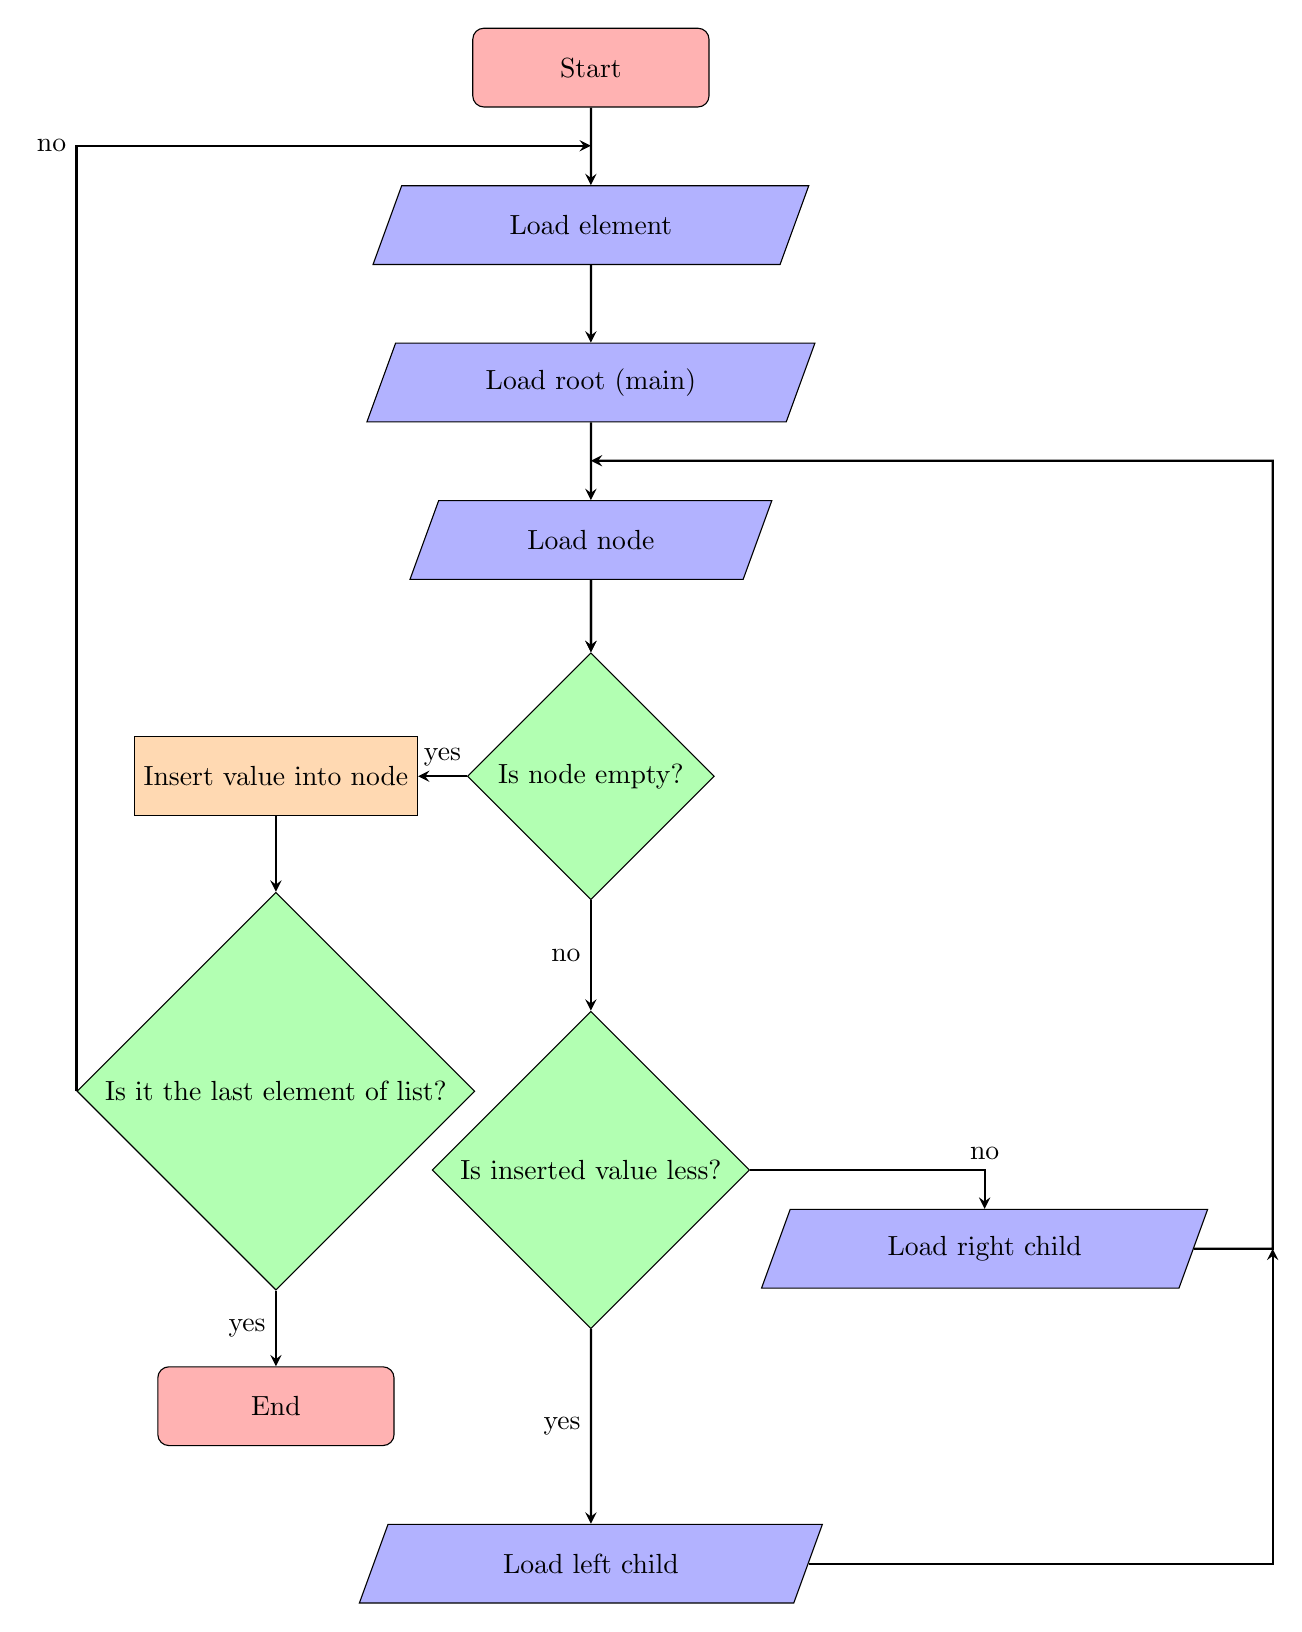
\begin{tikzpicture}[node distance=2cm]

    \node (start) [startstop] {Start};
    \node (load_list) [io, below of=start] {Load element};
    \node (load_root) [io, below of=load_list] {Load root (main)};
    \node (load_node) [io, below of=load_root] {Load node};
    \node (is_empty) [decision, below of=load_node, yshift=-1cm] {Is node empty?};
    \node (insert_value) [process, left of=is_empty, xshift=-2cm] {Insert value into node};
    \node (is_last) [decision, below of=insert_value, yshift=-2cm] {Is it the last element of list?};
    \node (end) [startstop, below of=is_last, yshift=-2cm] {End};
    \node (is_less) [decision, below of=is_empty, yshift=-3cm] {Is inserted value less?};
    \node (load_left) [io, below of=is_less, yshift=-3cm] {Load left child};
    \node (load_right) [io, right of=is_less, xshift=3cm, yshift=-1cm] {Load right child};

    \coordinate (node0) at ($(load_node.north)+(0,0.5cm)$);
    \coordinate (node1) at ($(load_right.east)+(1,0cm)$);
    \coordinate (node2) at ($(load_list.north)+(0,0.5cm)$);

    \draw [arrow] (start) -- (load_list);
    \draw [arrow] (load_list) -- (load_root);
    \draw [arrow] (load_root) -- (load_node);
    \draw [arrow] (load_node) -- (is_empty);
    \draw [arrow] (insert_value) -- (is_last);
    \draw [arrow] (load_node) -- (is_empty);
    \draw [arrow] (is_empty) -- node[anchor=south] {yes} (insert_value);
    \draw [arrow] (is_empty) -- node[anchor=east] {no} (is_less);
    \draw [arrow] (is_last) -- node[anchor=east] {yes} (end);
    \draw [arrow] (is_less.east) -| node[anchor=south] {no} (load_right.north);
    \draw [arrow] (is_less.south) -- node[anchor=east] {yes} (load_left.north);

    \draw [arrow] (load_right) -- (node1) |- (node0.east);
    \draw [arrow] (load_left) -| (node1);
    \draw [arrow] (is_last.west) |- node[anchor=east]{no}(node2);
\end{tikzpicture}


\end{document}